\documentclass[10pt]{beamer}

\usetheme[progressbar=frametitle]{metropolis}
\usepackage{appendixnumberbeamer}

\usepackage{booktabs}
\usepackage[scale=2]{ccicons}

\usepackage{pgfplots}
\usepgfplotslibrary{dateplot}

\usepackage{xspace}
\newcommand{\themename}{\textbf{\textsc{metropolis}}\xspace}

\usepackage{verbatim}

\title{Hierarchical Solutions for the Stochastic Block Model}
\author{Aditi Nair and Akash Shah}
% \titlegraphic{\hfill\includegraphics[height=1.5cm]{logo.pdf}}

\begin{document}

\maketitle

\begin{frame}
\frametitle{The Stochastic Block Model}
\begin{itemize}
\item{Let $G$ be a graph with $k$ communities of $m$ nodes each}
\item{For nodes $(i,j)$ in the same community, let the $p$ be the probability that they share an edge on $G$}
\item{For nodes $(i,j)$ not in the same community, let the $q$ be the probability that they \textit{don't} share an edge on $G$}
\item{Edges are drawn independently, and $p>q$}
\item{Goal: recover the original partition}
\end{itemize}
\end{frame}

\begin{frame}
\frametitle{The Semidefinite Program for $k=2$}
Let $A$ be the adjacency matrix of $G$. Then we need to solve:
$$\max \sum_{i,j} A_{ij} x_{i} x_{j} $$
$$ \text{s.t. } x_i = \pm 1 \ \forall i$$
$$\sum_j x_j = 0$$
\end{frame}

\begin{frame}
\frametitle{The Semidefinite Program for $k=2$}
Let $B = 2A - (\textbf{1}\textbf{1}^T - I)$. Then the original problem is equivalent to
$$\max \sum_{i,j} B_{ij} x_{i} x_{j} $$
$$ \text{s.t. } x_i = \pm 1 \ \forall i$$
$$\sum_j x_j = 0$$
\end{frame}

\begin{frame}
\frametitle{The Semidefinite Program for $k=2$}
By dropping the constraint $\sum_j x_j = 0$ and with a convex relaxation, we have the following semidefinite program:
$$\max Tr(BX)$$
$$ \text{s.t. } X_{ii}= 1 \ \forall i$$
$$X \succeq 0$$
Under the right conditions, with high probability the solution coincides with $X=gg^{T}$. We obtain $g$ by finding the leading eigenvector of $X$.
\end{frame}

\begin{frame}
\frametitle{Conditions for Recovery}
\begin{tabular}{c | c | c }
 & Exact & Partial \\ \hline
 Formula & $p = \frac{\alpha \log n}{n}$, $q = \frac{\beta \log n}{n}$ & $p = \frac{a}{n}$, $q = \frac{b}{n}$ \\ \hline
$k = 2$ & $\sqrt{\alpha} - \sqrt{\beta} \geq \sqrt{2}$ & $(a-b)^2 > 2(a+b)$ \\ 
$k > 2$ &  $\sqrt{\alpha} - \sqrt{\beta} \geq \sqrt{k}$ & $\frac{(a-b)^2}{k(a+(k-1)b)} > 1$ \\ \hline
 \end{tabular}
\end{frame}

\begin{frame}
\frametitle{Hierarchical Approach for $k>2$}

\begin{figure}
  \centering
 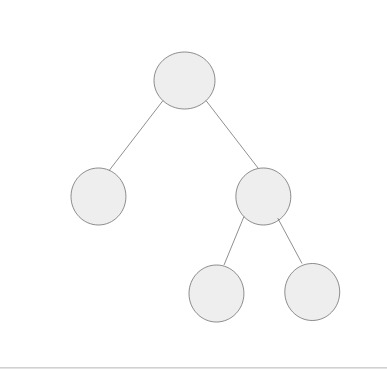
\includegraphics[scale=0.9]{three_comm.jpg}
 \caption{Hierarchy for k = 3}
\end{figure}

\begin{figure}
  \centering
 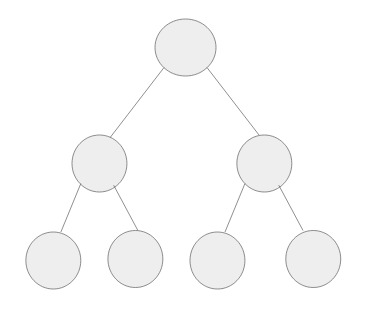
\includegraphics[scale=.9]{four_comm.jpg}
 \caption{Hierarchy for k = 4}
\end{figure}

\end{frame}

\begin{frame}
\frametitle{Exact Recovery for $k=2$}
\begin{figure}
  \centering
 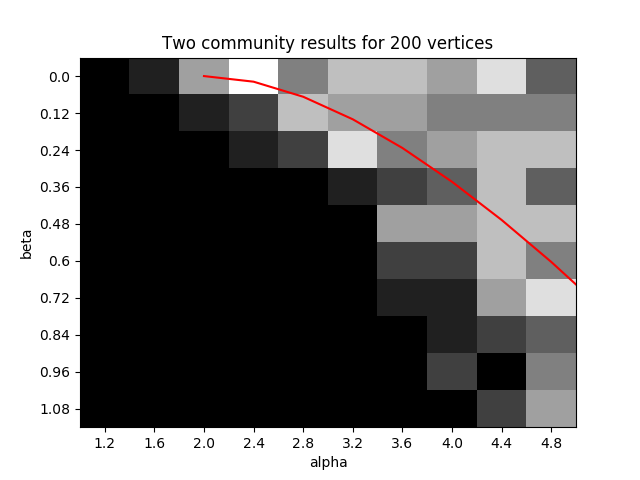
\includegraphics[scale=.6]{../exact/final_plots/two_community_200_verts.png}
\end{figure}

\end{frame}

\begin{frame}
\frametitle{Exact Recovery for $k=3$}
\begin{figure}
  \centering
 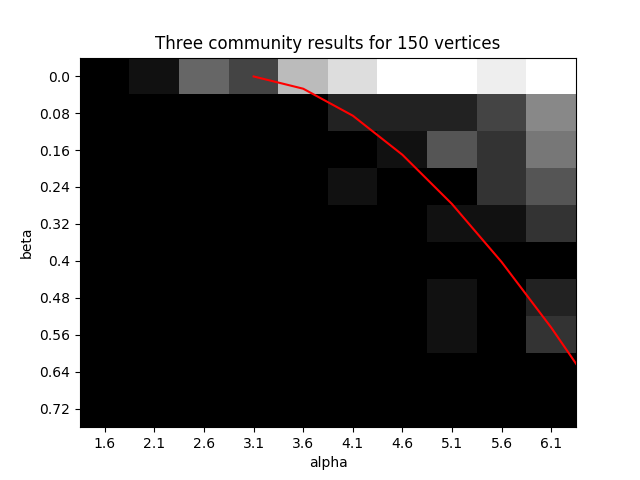
\includegraphics[scale=.6]{../exact/final_plots/three_communities_150_verts.png}
\end{figure}

\end{frame}

\begin{frame}
\frametitle{Exact Recovery for $k=4$}
\begin{figure}
  \centering
 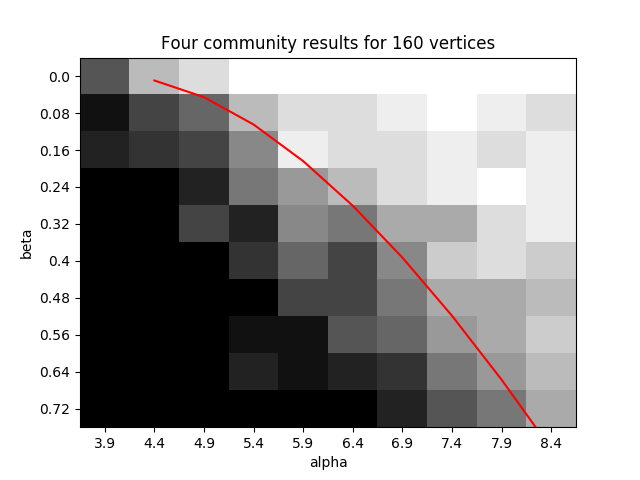
\includegraphics[scale=.6]{../exact/final_plots/four_communities_160_verts.png}
\end{figure}

\end{frame}

\begin{frame}
\frametitle{Partial Recovery for $k=2$}
\begin{figure}
  \centering
 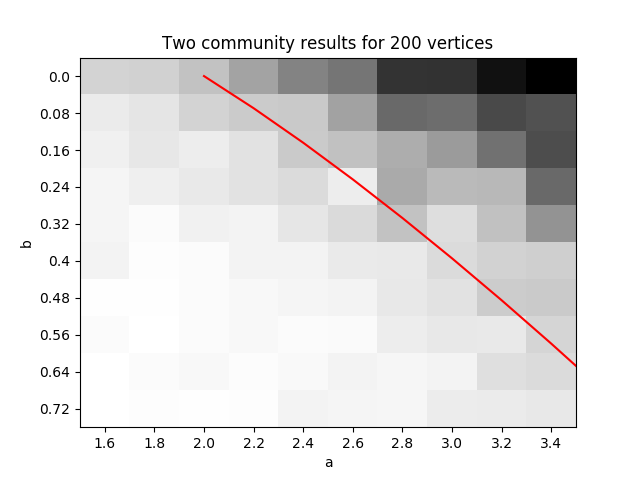
\includegraphics[scale=.6]{../inexact/final_plots/two_communities_200_verts.png}
\end{figure}

\end{frame}

\begin{frame}
\frametitle{Partial Recovery for $k=3$}
\begin{figure}
  \centering
 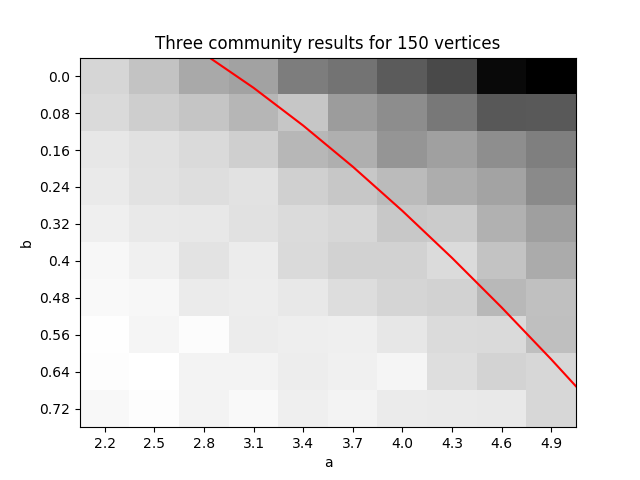
\includegraphics[scale=.6]{../inexact/final_plots/three_communities_150_verts.png}
\end{figure}
\end{frame}

\begin{frame}
\frametitle{Partial Recovery for $k=4$}
\begin{figure}
  \centering
 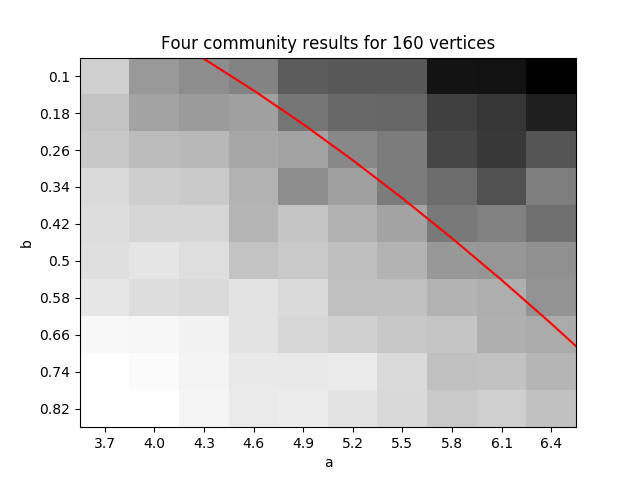
\includegraphics[scale=.6]{../inexact/final_plots/four_communities_160_verts.png}
\end{figure}
\end{frame}

\end{document}
